\section{Laboratory Lecture 3: Temperature Measuring using the LM35 sensor.}

The aim of this laboratory lecture is to design an ATMega328P-based temperature measurement system. This system will read an analog voltage, provided by the LM35, which will be proportional to the ambient temperature, and it will show it on a 16x2 LCD. \medskip

\subsection{Introduction}

Before diving into the laboratory lecture itself, some of the concepts related to it must be firstly explained, namely interrupts, the analog comparator and the analog-to-digital converter.

\subsubsection{Interrupts}

When monitoring the state of a signal is needed in a project, two different strategies can be followed.\medskip

The first, and most inneficient is called \textbf{Polling}. \textbf{Polling} consists in checking the state of the pin/port continuously, i.e. at a specific part of the code in every run. This can cause delays and in general, is not efficient, as the microcontroller needs to constantly check the state of the pin, making the execution of the code slower.\medskip

On the other hand, we find \textbf{Interrupts}. An \textbf{interrupt} can be defined as an internal mechanism of the microcontroller that allows it to interrupt the execution of the code when a specific internal or external event occurs. Once the interrupt is triggered, the microcontroller enters in what is called an interrupt subroutine, which is a small chunk of code that only gets executed when the interrupt is triggered and that remains \textit{invisible} to the rest of the code, avoiding in this way the efficiency problems that polling posed. Once the interrupt subroutine is finished, the execution of the main code is resumed at the exact place where it was interrupted. \medskip

\clearpage

This behaviour can be seen on the image below:

\begin{figure}[H]
    \centering
    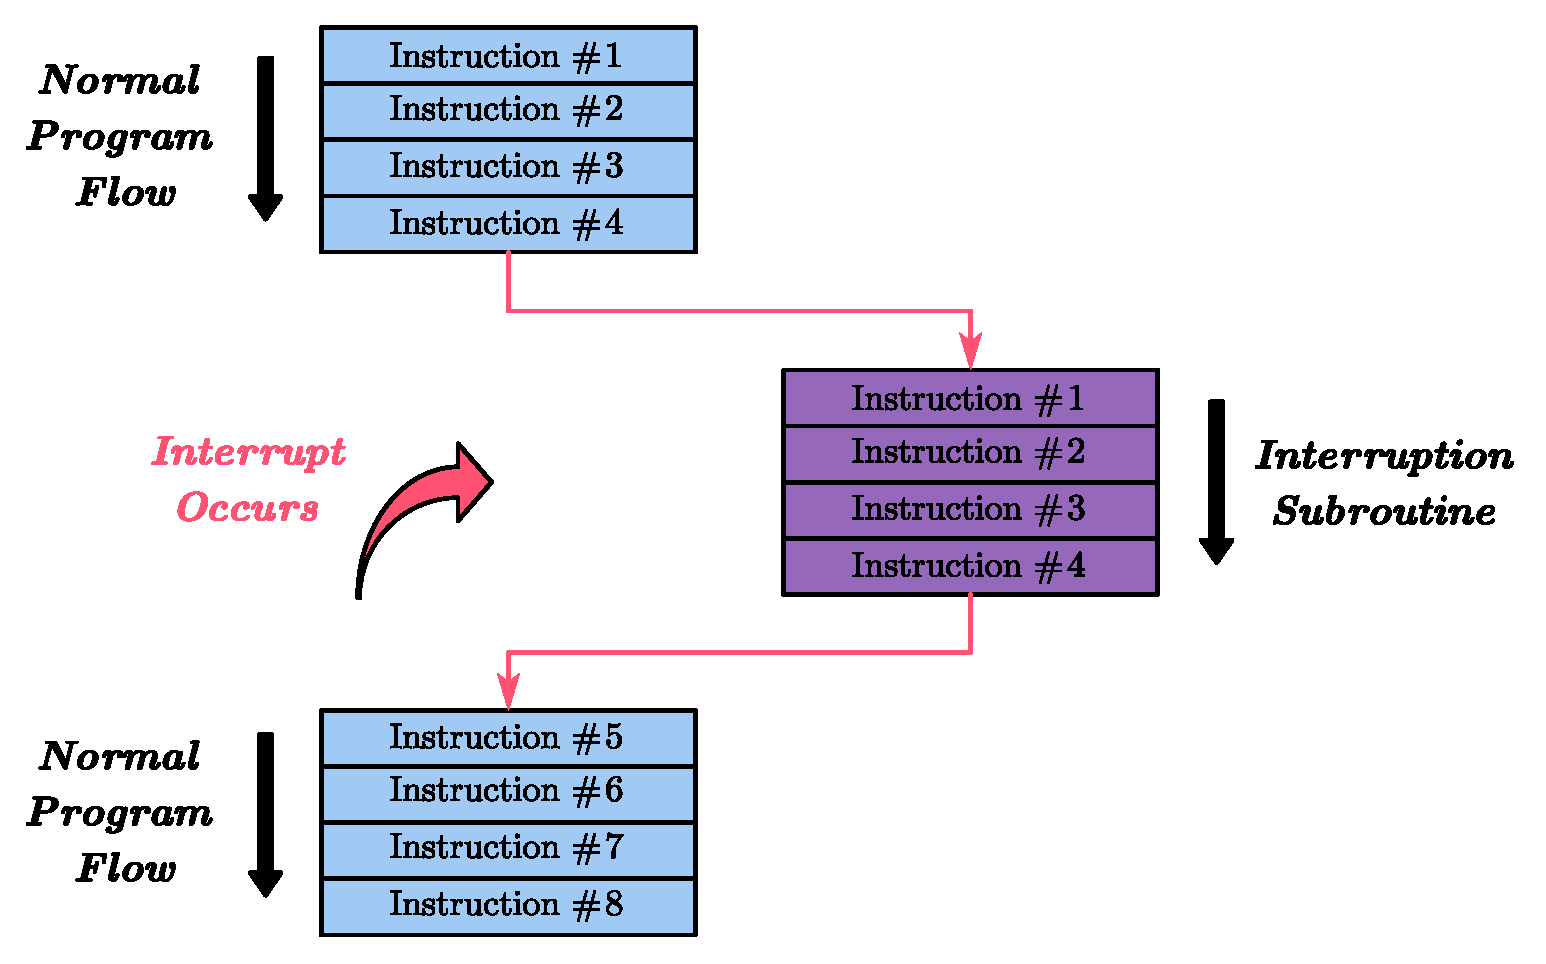
\includegraphics[scale = 0.5]{Graphics/MICROS/Practice 3/Interrup_Flow_Chart.pdf}
    \caption{Interruption Subroutine Flowchart}
    \label{fig:ISR_FLOWCHART}
\end{figure}

The ATMega328P has 26 interrupt sources:~\autocite{SLIDES_MICROS}

\begin{itemize}
    \item 1 Reset source.
    \item 2 External Interrupt sources (Sense control).
    \item 24 External Interrupt sources (Only triggered by I/O change).
    \item Peripheral Device Events (ADC, AC, Timers)
\end{itemize}

\paragraph{Enabling Interrupts}

To enable the interrupts, the Global Interrupt Enable Bit, in the SREG register, must be set. We can see this here:

\begin{figure}[H]
    \centering
    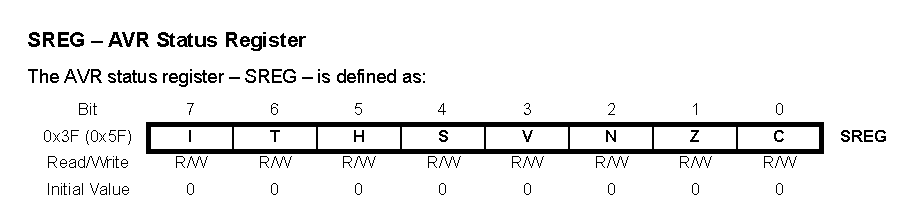
\includegraphics[width = \textwidth]{Graphics/MICROS/Practice 3/DATASHEET/SREG.pdf}
    \caption{AVR Status Register~\autocite{ATMEGA328P}}
    \label{fig:SREG}
\end{figure}

\clearpage

When an interrupt is triggered, the ISR (Interrupt Service Routine) is called, the execution of the main code is stopped, and the Global Interrupt Enable Bit is automatically cleared. When the interrupt ends, the RETI, which is added at the end of every ISR by default, sets the Global Interrupt Enable Bit to 1 and the execution of the code is resumed. \medskip

The ISR should NOT involve neither extensive computations nor complicates loops.\medskip

A basic C program showing the basics of ISRs can be found below:

\inputCcode{CODES/MICROS/Practice_3/EXPLANATION/ISR_basics.c}


\paragraph{Types of Interrupts}

There are 2 main types of interrupts, namely:

\begin{enumerate}
    \item \textbf{Type I:} Event is remembered when GIEB is cleared.
        \begin{itemize}
            \item A flag is set when the interrupt is not enabled. When it is enabled again the ISR takes place.
        \end{itemize}

    \item \textbf{Type II:} Event is NOT remembered when GIEB is cleared.
        \begin{itemize}
            \item If the event occurs when the interrupts are enabled, the ISR takes place, otherwise it does not.
        \end{itemize}
\end{enumerate}

If the interrrupts are not used in a project, their allocated memory can be used by the rest of the program.~\autocite{SLIDES_MICROS}


\paragraph{External Interrupts: INT0-INT1}

As we said before the ATMega328P has 2 external interrupts which sense, i.e. how they are triggered, can be configured. The other 24 can only be triggered when the state of a pin changes.\medskip

To control the first two, the \textbf{External Interrupt Control Register}, \textbf{EICRA} for short, must be configured.

\begin{figure}[H]
    \centering
    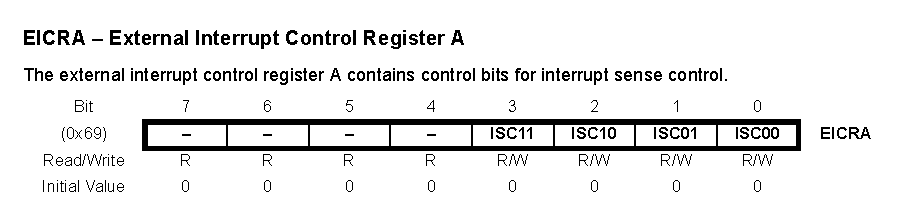
\includegraphics[width = \textwidth]{Graphics/MICROS/Practice 3/DATASHEET/EICRA.pdf}
    \caption{External Interrupt Control Register~\autocite{ATMEGA328P}}
    \label{fig:EICRA}
\end{figure}

As we can see, the last 4 bits control the INT1 and INT0, respectively. A table showcasing all of the possible configurations, in this case for INT1, though the same applies to INT0, can be found below:


\begin{table}[H]
    \resizebox{\columnwidth}{!}{
        \centering
        \begin{tabular}[t]{lccc}
            \toprule
            & \textbf{ISC11} & \textbf{ISC10} & \textbf{Description} \\
            \midrule
            & 0 & 0 & The LOW level of INT1 generates an interrupt request.                                                              \\
            & 0 & 1 & Any logical change on INT1 generates an interrupt request.  \\
            & 1 & 0 & The falling edge of INT1 generates an interrupt request.                                                              \\
            & 1 & 0 & The rising edge of INT1 generates an interrupt request.                                                               \\

            \bottomrule
        \end{tabular}
        \caption{INT1 Sense Control.~\autocite{ATMEGA328P}}
        \label{table:INT1_SENSE_CONTROL}
        }
\end{table}



\begin{figure}[H]
    \centering
    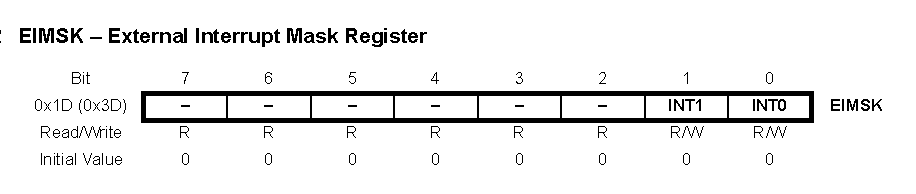
\includegraphics[width = \textwidth]{Graphics/MICROS/Practice 3/DATASHEET/EIMSK.pdf}
    \caption{External Interrupt Mask Register~\autocite{ATMEGA328P}}
    \label{fig:EIMSK}
\end{figure}

To enable the interrupts, apart from setting the Global Interrupt Enable Bit in the SREG to 1, the \textbf{INT\#} in the \textbf{External Interrupt Mask Register}, \textbf{EIMSK} for short, must be set. If this bit is set, then INT\# will be enabled.\medskip


\begin{figure}[H]
    \centering
    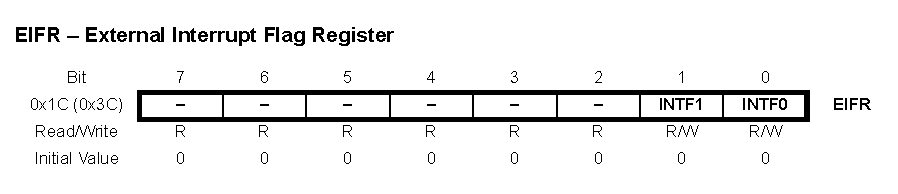
\includegraphics[width = \textwidth]{Graphics/MICROS/Practice 3/DATASHEET/EIFR.pdf}
    \caption{External Interrupt Flag Register~\autocite{ATMEGA328P}}
    \label{fig:EIFR}
\end{figure}

Finally, we also find the \textbf{External Interrupt Flag Register}, \textbf{EIFR} for short. The last 2 bits of this register, INTF1 and INTF0 respectively, show when an ISR is being executed. The corresponding bit is set to 1 while the ISR is being executed, and is cleared after its execution.\medskip


\paragraph{External Interrupts: PCINT[23:0]}

Apart from the 2 external interrupts that we have just discussed, there are 24 more interrupts available to the user, one for each GPIO pin. The only drawback that these external interrupts have is the fact that their sense, i.e. how they are triggered, cannot be selected, as they only trigger on a change of pin state.\medskip

To control these interrupts, we have to resort to the datasheet. In in, we find that this control is performed by 3 different registers:

\begin{figure}[H]
    \centering
    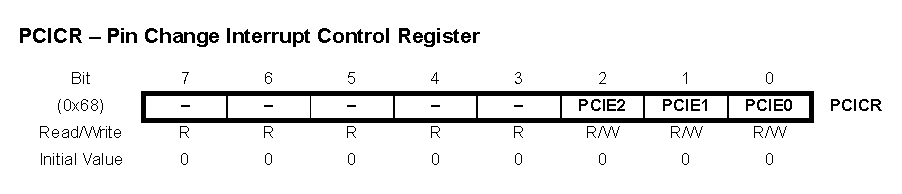
\includegraphics[width = \textwidth]{Graphics/MICROS/Practice 3/DATASHEET/PCICR.pdf}
    \caption{Pin Change Interrupt Control Register~\autocite{ATMEGA328P}}
    \label{fig:PCICR}
\end{figure}

The last 3 bits of the \textbf{Pin Change Interrupt Control Register}, or \textbf{PCICR} for short, enable the interrupts following this fashion:

\begin{itemize}
    \item \textbf{PCIE2:} A 1 in this bit enables the interrupts form PCINT[23:16]
    \item \textbf{PCIE1:} A 1 in this bit enables the interrupts form PCINT[14:8]
    \item \textbf{PCIE0:} A 1 in this bit enables the interrupts form PCINT[7:0]
\end{itemize}

\clearpage

After setting the corresponding bits on this register, the interrupt mask must also be enabled.\medskip

\begin{figure}[H]
    \centering
    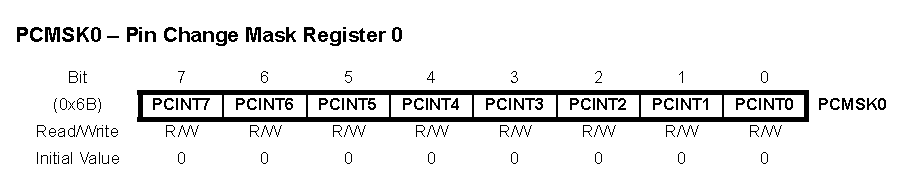
\includegraphics[width = \textwidth]{Graphics/MICROS/Practice 3/DATASHEET/PCMSK0.pdf}
    \caption{Pin Change Mask Register 0~\autocite{ATMEGA328P}}
    \label{fig:PCMSK0}
\end{figure}

\vspace{-0.5cm}

\begin{figure}[H]
    \centering
    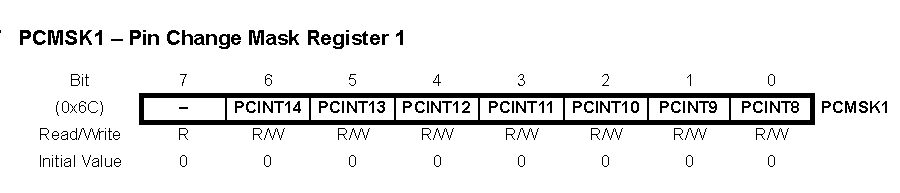
\includegraphics[width = \textwidth]{Graphics/MICROS/Practice 3/DATASHEET/PCMSK1.pdf}
    \caption{Pin Change Mask Register 1~\autocite{ATMEGA328P}}
    \label{fig:PCMSK1}
\end{figure}

\vspace{-0.5cm}

\begin{figure}[H]
    \centering
    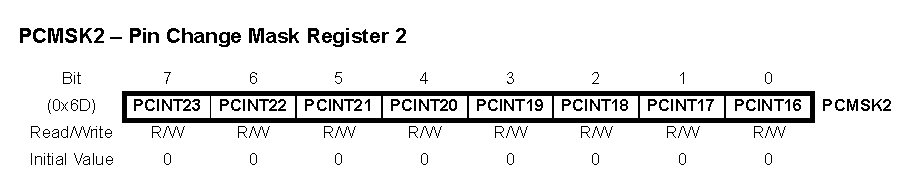
\includegraphics[width = \textwidth]{Graphics/MICROS/Practice 3/DATASHEET/PCMSK2.pdf}
    \caption{Pin Change Mask Register 2~\autocite{ATMEGA328P}}
    \label{fig:PCMSK2}
\end{figure}


To do this, we will modify the state of some of the bits belonging to the \textbf{Pin Change Mask Register n}, or \textbf{PCMSKn} for short. \textbf{n} corresponds to the number of the \textbf{PCIEn}, i.e., PCMSK1 is an 8-bit register that controls the PCINT[14:8] interrupts. 


\begin{figure}[H]
    \centering
    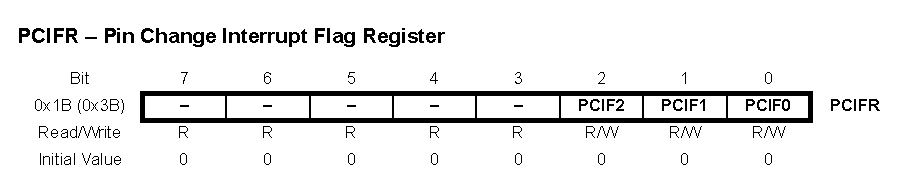
\includegraphics[width = \textwidth]{Graphics/MICROS/Practice 3/DATASHEET/PCIFR.pdf}
    \caption{Pin Change InterruptFlag Register~\autocite{ATMEGA328P}}
    \label{fig:PCIFR}
\end{figure}

Finally, as in the INT0-INT1 registers, we have the \textbf{Pin Change Interrupt Flag Register}, or \textbf{PCIFR} for short. PCIF\# will be set whenever an interrupt request occurs and will be cleared once it is processed.


\subsubsection{Peripheral Modules}

All AVR microcontrollers, including the ATMega328P, have 2 peripherals which are resposible for handling analog data.~\autocite{SLIDES_MICROS}

\begin{itemize}
    \item \textbf{Analog Comparator (AC):} Two analog inputs, AIN0 and AIN1, are compared. A bit indicates if AIN0 is greater than AIN1.
    \item \textbf{Analog-to-Digital Converter (ADC):} It generates a 10-bit number which is proportional to the amplitude of the input signal (0-1023).
\end{itemize}

\paragraph{Analog Comparator}

The Analog Comparator is, in essence, an open loop operational amplifier which $V_{+}$ and $V_{-}$ terminals can be connected to multiple input signals.\medskip

It can act as a mere comparator, i.e., comparing the AIN0 signal to the AIN1, in which case the output will be 1 if AIN0$\; > \;$AIN1, though an internal reference voltage of 1.1 V can replace AIN0, making it a comparator with a fixed reference.\medskip

AIN1, on the other hand, can also be replaced by a multiplexed signal coming from the ADC, i.e., by any of the ADC ports, making it possible to compare more than one analog signal with the same reference. For this, the ADC must be disabled.\medskip

An image showing the internal configuration of the Analog Comparator can be seen below:

\begin{figure}[H]
    \centering
    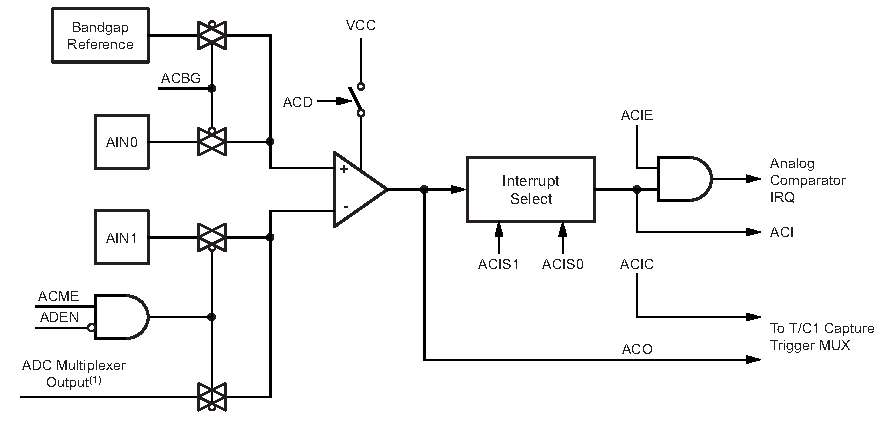
\includegraphics[width = \textwidth]{Graphics/MICROS/Practice 3/DATASHEET/AC_BLOCK_DIAGRAM.pdf}
    \caption{Analog Comparator Block Diagram~\autocite{ATMEGA328P}}
    \label{fig:AC_BLOCK_DIAGRAM}
\end{figure}

\clearpage

\medskip
\underline{\textbf{Basic Comparator}}
\medskip

As we said before, the Analog Comparator can work as a basic open loop comparator. In this way, whenever the AIN0 voltage exceeds the AIN1 voltage, the \textbf{ACO} bit will be set to 1.\medskip

This output can generate an interruption if it is configured to do so in the \textbf{Analog Comparator Control and Status Register}, \textbf{ACSR} for short. 

\begin{figure}[H]
    \centering
    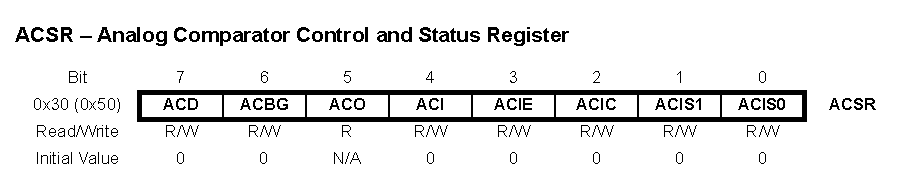
\includegraphics[width = \textwidth]{Graphics/MICROS/Practice 3/DATASHEET/ACSR.pdf}
    \caption{Analog Comparator Control and Status Register~\autocite{ATMEGA328P}}
    \label{fig:ACSR}
\end{figure}


\begin{table}[H]
        \centering
        \begin{tabular}[t]{lccc}
            \toprule
            & \textbf{ACIS1} & \textbf{ACIS0} & \textbf{Interrupt Mode}      \\
            \midrule
            & 0 & 0 & Comparator Interrupt on Output Toggle                  \\
            & 0 & 1 & Reserved                                               \\
            & 1 & 0 & Comparator Interrupt on Falling Output Edge            \\
            & 1 & 0 & Comparator Interrupt on Rising Output Edge             \\
            \bottomrule
        \end{tabular}
        \caption{Analog Comparator Interrupt Mode Select.~\autocite{ATMEGA328P}}
        \label{table:ACISn_COMP}
\end{table}

As we can see, by modifying the values of the last 2 bits, the \textbf{Analog Comparator Interrupt Mode Select}, or \textbf{ACIS} bits for short, the comparator can behave in different ways.

\clearpage

\medskip
\underline{\textbf{Bandgap Reference}}
\medskip

The \textbf{AIN0} input can be replaced by a fixed bandgap reference voltage of 1.1 V. To do so, the \textbf{Analog Comparator Bandgap Select}, \textbf{ACBG} for short, bit in the \textbf{ACSR} Register (Figure \ref{fig:ACSR}) must be set to 1.\medskip

This register includes other important bits that must be set to either one or zero to ensure a proper operation of the AC.

\begin{itemize}
    \item \textbf{Bit 7 - ACD: Analog Comparator Disable:} When this bit is written logic one, the power to the analog comparator is switched off. This bit can be set at any time to turn
    off the analog comparator.

    \item \textbf{Bit 5 – ACO: Analog Comparator Output:} The output of the analog comparator is synchronized and then directly connected to ACO. The synchronization introduces a
    delay of 1 - 2 clock cycles.

    \item \textbf{Bit 4 – ACI: Analog Comparator Interrupt Flag:} This bit is set by hardware when a comparator output event triggers the interrupt mode defined by ACIS1 and ACIS0. The
    analog comparator interrupt routine is executed if the ACIE bit is set and the I-bit in SREG is set. ACI is cleared by hardware when executing the corresponding interrupt handling vector. Alternatively, ACI is cleared by writing a logic one to the flag.

    \item \textbf{Bit 3 – ACIE: Analog Comparator Interrupt Enable:} When the ACIE bit is written logic one and the I-bit in the status register is set, the analog comparator interrupt is activated. When written logic zero, the interrupt is disabled.
    
    \item \textbf{Bit 2 – ACIC: Analog Comparator Input Capture Enable:} When written logic one, this bit enables the input capture function in Timer/Counter1 to be triggered by the analog
    comparator. The comparator output is in this case directly connected to the input capture front-end logic, making the comparator utilize the noise canceler and edge select features of the Timer/Counter1 input capture interrupt. When written logic zero, no connection between the analog comparator and the input capture function exists. To make the comparator trigger the Timer/Counter1 input capture interrupt, the ICIE1 bit in the timer interrupt mask register (TIMSK1) must be set.
    
\end{itemize}

\clearpage

\medskip
\underline{\textbf{ADC Input}}
\medskip


Finally, the \textbf{AIN1} input can also be replaced by one of the multiplexed ADC inputs. To do so, the ACD must be disabled and the MUX must be enabled.\medskip

To disable the ADC, the \textbf{ADC Enable} bit, \textbf{ADEN} for short, in the \textbf{ADC Control and Status Register A}, \textbf{ADCSRA} for short, must be set to \textbf{0}. \medskip

This last register can be seen below:

\begin{figure}[H]
    \centering
    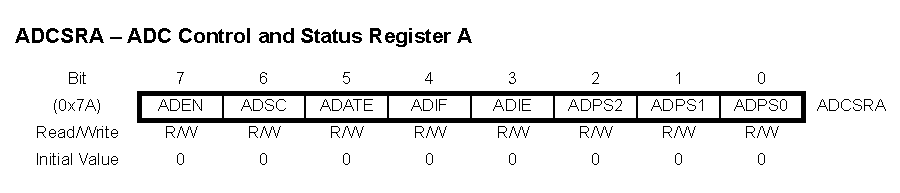
\includegraphics[width = \textwidth]{Graphics/MICROS/Practice 3/DATASHEET/ADCSRA.pdf}
    \caption{ADC Control and Status Register A~\autocite{ATMEGA328P}}
    \label{fig:ADCSRA}
\end{figure}


On the other hand, to enable the MUX, the \textbf{Analog Comparator Multiplexer Enable} bit, \textbf{ACME} for short, in the \textbf{ADC Control and Status Register B}, \textbf{ADCSRB} for short, must be set to 1.\medskip

The mentioned register can be seen below:

\begin{figure}[H]
    \centering
    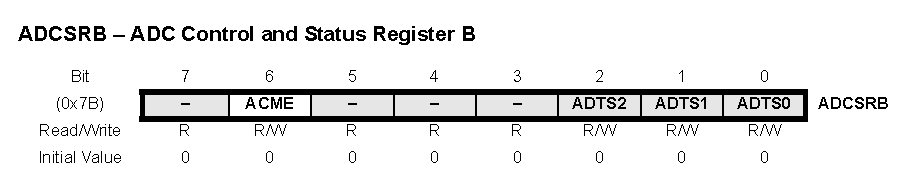
\includegraphics[width = \textwidth]{Graphics/MICROS/Practice 3/DATASHEET/ADCSRB.pdf}
    \caption{ADC Control and Status Register B~\autocite{ATMEGA328P}}
    \label{fig:ADCSRB}
\end{figure}


Once the MUX is enabled, to select the input channel, the MUX[3:0] bits in the \textbf{ADC Multiplexer Selection Register}, \textbf{ADMUX} for short must be set accordingly to the following table:

\begin{table}[H]
        \centering
        \begin{tabular}[t]{lcc}
            \toprule
            & \textbf{MUX[3:0]} & \textbf{Single Ended Input} \\
            \midrule
            & 0000 & ADC0  \\
            & 0001 & ADC1  \\
            & 0010 & ADC2  \\
            & 0011 & ADC3  \\
            & 0100 & ADC4  \\
            & 0101 & ADC5  \\
            & 0110 & ADC6  \\
            & 0111 & ADC7  \\
            \bottomrule
        \end{tabular}
        \caption{MUXn Input Channel Selection~\autocite{ATMEGA328P}}
        \label{table:MUXN_SELECTION}
\end{table}

\medskip
\underline{\textbf{Input Disable}}
\medskip

To disable the AIN0 or AIN1 inputs, a 1 must be written to the corresponding, \textbf{AINx Digital Input Disable} bit, \textbf{AINxD} for short, which belongs to the \textbf{DIDR1} register.

\begin{figure}[H]
    \centering
    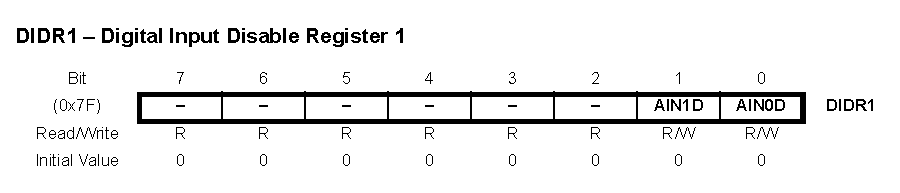
\includegraphics[width = \textwidth]{Graphics/MICROS/Practice 3/DATASHEET/DIDR1.pdf}
    \caption{Digital Input Disable Register 1~\autocite{ATMEGA328P}}
    \label{fig:DIDR1}
\end{figure}



\paragraph{Analog-to-Digital Converter}

The Analog-to-Digital Converter is a peripheral that takes an input analog signal and translates it into the digital spectrum.

\begin{figure}[H]
    \centering
    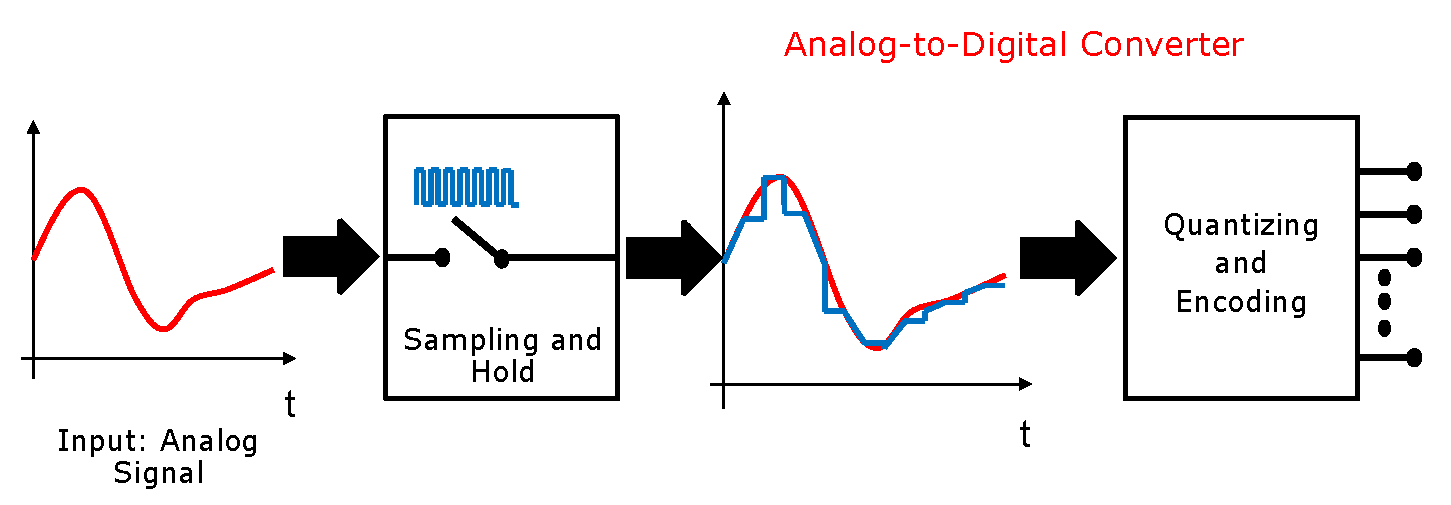
\includegraphics[width = \textwidth]{Graphics/MICROS/Practice 3/DATASHEET/ADC_DIAGRAM.pdf}
    \caption{ADC Processes Diagram~\autocite{ADC_PROCESS}}
    \label{fig:ADC_DIAGRAM}
\end{figure}

As it can be seen in the image, every ADC conversion can be broken down into 3 individual processes:

\begin{enumerate}
    \item \textbf{Sample \& Hold:} Which is performed by an auxiliary device which purpose is to capture the input voltage and hold it for a specified minimal period of time.
    \item \textbf{Quantization:} Is the process of converting a continuous range of values into a finite range of discreet values. This is a function of analog-to-digital converters, which create a series of digital values to represent the original analog signal. 
    \item \textbf{Codification:} Consists of the translation of the analogical values of tension electrical that already have been quantified (averaged) to binary system, by means of pre-established codes.
\end{enumerate}

The ATMega328 includes an ADC of successive approximations of 10 bits, the result of the conversion is stored in two I/O registers: \textbf{ADCH} and \textbf{ADCL} (in Language C the pair can be treated as \textbf{ADCW}).\medskip

Since there is only 1 ADC, the analog inputs have to be multiplexed. This results in 8 external channels, namely ADC[7:0], though in the P DIP package of the ATMega328P, only 6 are available.\medskip

To reach the maximum resolution, the ADC must work with a frequency between 50 and 200 kHz, which can be generated with a pre-scaler, starting from the base frequency of the microcontroller.\medskip

The first conversion requires initializing the analog circuitry, so it invests 25 clock cycles. The following conversions only use 13 clock cycles.\medskip

There are 4 8-bit registers that control the ADC:

\begin{enumerate}
    \item \textbf{ADCSRA} - ADC Control and Status Register A
    \item \textbf{ADCSRB} - ADC Control and Status Register B
    \item \textbf{ADMUX}  - ADC Multiplexer Selection Register
    \item \textbf{DIDR0}  - Digital Input Disable Register 0
\end{enumerate}

\medskip
\underline{\textbf{ADCSRA}}
\medskip

The \textbf{ADC Control and Status Register A}, or \textbf{ADCSRA} for short, controls the basic operations of the ADC. In it, there are 8 bits that must be configured to make the ADC work properly. These bits are:

\begin{figure}[H]
    \centering
    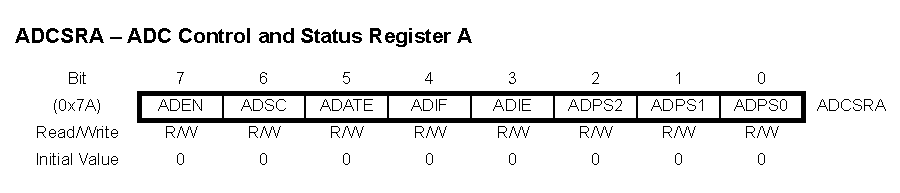
\includegraphics[width = \textwidth]{Graphics/MICROS/Practice 3/DATASHEET/ADCSRA.pdf}
    \caption{ADC Control and Status Register A~\autocite{ATMEGA328P}}
    \label{fig:ADCSRA}
\end{figure}


\begin{itemize}
    \item \textbf{Bit 7 – ADEN: ADC Enable} $\bm{\rightarrow}$  Writing this bit to one enables the ADC. By writing it to zero, the ADC is turned off. Turning the ADC off while a conversion is in progress, will terminate this conversion.
    
    \item \textbf{Bit 6 – ADSC: ADC Start Conversion} $\bm{\rightarrow}$ In single conversion mode, write this bit to one to start each conversion. In free running mode, write this bit to one to start the
    first conversion. ADSC will read as one as long as a conversion is in progress. When the conversion is complete, it returns to zero.

    \item \textbf{Bit 5 – ADATE: ADC Auto Trigger Enable} $\bm{\rightarrow}$ When this bit is written to one, auto triggering of the ADC is enabled. The ADC will start a conversion on a positive edge of the selected trigger signal. The trigger source is selected by setting the ADC trigger select bits, ADTS in ADCSRB.
    
    \item \textbf{Bit 5 – ADIF: ADC Interrupt Flag} $\bm{\rightarrow}$ This bit is set when an ADC conversion completes and the data registers are updated. The ADC conversion complete interrupt is executed if the ADIE bit and the GIEB (I-Bit) in SREG are set. ADIF is cleared by hardware when executing the corresponding interrupt handling vector. Alternatively, ADIF is cleared by writing a logical one to the flag. Beware that if doing a read-modify-write on ADCSRA, a pending interrupt can be disabled. This also applies if the SBI and CBI instructions are used.
    
    \item \textbf{Bit 3 – ADIE: ADC Interrupt Enable} $\bm{\rightarrow}$ When this bit is written to one and the GIEB (I-bit) in SREG is set, the ADC conversion complete interrupt is activated.
    
    \item \textbf{Bits [2:0] – ADPS[2:0]: ADC Prescaler Select Bits} $\bm{\rightarrow}$ These bits determine the division factor between the system clock frequency and the input clock to the ADC.
    
\end{itemize}

\begin{table}[H]
    \centering
    \begin{tabular}[t]{lcccc}
        \toprule
        & \textbf{ADPS2} & \textbf{ADPS1} & \textbf{ADPS0} & \textbf{Division Factor}\\
        \midrule
        & 0 & 0 & 0 & 2   \\
        & 0 & 0 & 1 & 2   \\
        & 0 & 1 & 0 & 4   \\
        & 0 & 1 & 1 & 8   \\
        & 1 & 0 & 0 & 16  \\
        & 1 & 0 & 1 & 32  \\
        & 1 & 1 & 0 & 64  \\
        & 1 & 1 & 1 & 128 \\
        \bottomrule
    \end{tabular}
    \caption{ADC Prescaler Selections~\autocite{ATMEGA328P}}
    \label{table:ADC_PRESCALER}
\end{table}

\clearpage

\medskip
\underline{\textbf{ADCSRB}}
\medskip

The \textbf{ADC Control and Status Register B}, or \textbf{ADCSRB} for short, is mainly used to select the trigger souce of the ADC. There are 3 bits that must be configured to make the ADC work properly. These bits are:

\begin{figure}[H]
    \centering
    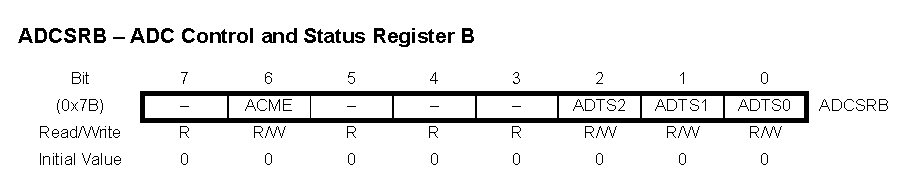
\includegraphics[width = \textwidth]{Graphics/MICROS/Practice 3/DATASHEET/ADCSRB_2.pdf}
    \caption{ADC Control and Status Register B~\autocite{ATMEGA328P}}
    \label{fig:ADCSRB}
\end{figure}

\begin{itemize}
    \item \textbf{Bit 2:0 – ADTS2:0: ADC Auto Trigger Source} $\bm{\rightarrow}$ If \textbf{ADATE} in \textbf{ADCSRA} is written to one, the value of these bits selects which source will trigger an ADC conversion. If \textbf{ADATE} is cleared, the \textbf{ADTS[2:0]} settings will have no effect. A conversion will be triggered by the rising edge of the selected interrupt flag. Note that switching from a trigger source that is cleared to a trigger source that is set, will generate a positive edge on the trigger signal. If \textbf{ADEN} in \textbf{ADCSRA} is set, this will start a conversion. Switching to free running mode (\textbf{ADTS[2:0]=0}) will not cause a trigger event, even if the ADC interrupt flag is set.
\end{itemize}


\begin{table}[H]
    \centering
    \begin{tabular}[t]{lcccc}
        \toprule
        & \textbf{ADTS2} & \textbf{ADTS1} & \textbf{ADTS0} & \textbf{Trigger Source}\\
        \midrule
        & 0 & 0 & 0 & Free running mode               \\
        & 0 & 0 & 1 & Analog comparator               \\
        & 0 & 1 & 0 & External interrupt request 0    \\
        & 0 & 1 & 1 & Timer/Counter0 compare match A  \\
        & 1 & 0 & 0 & Timer/Counter0 overflow         \\
        & 1 & 0 & 1 & Timer/Counter1 compare match B  \\
        & 1 & 1 & 0 & Timer/Counter1 overflow         \\
        & 1 & 1 & 1 & Timer/Counter1 capture event    \\
        \bottomrule
    \end{tabular}
    \caption{ADC Prescaler Selections~\autocite{ATMEGA328P}}
    \label{table:ADC_PRESCALER}
\end{table}

\clearpage

\medskip
\underline{\textbf{ADMUX}}
\medskip

The \textbf{ADC Multiplexer Selection Register}, \textbf{ADMUX} for short, as its name implies, allows us to select the sources/references for the ADC. There are 7 bits that must be configured for a proper operation. These bits are:


\begin{figure}[H]
    \centering
    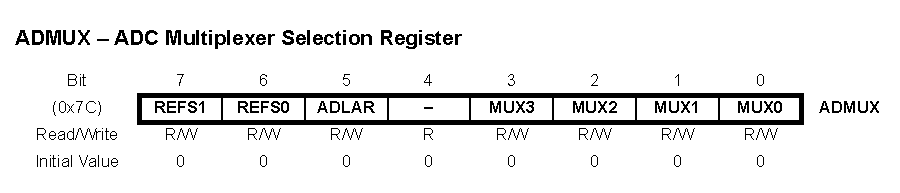
\includegraphics[width = \textwidth]{Graphics/MICROS/Practice 3/DATASHEET/ADMUX.pdf}
    \caption{ADC Multiplexer Selection Register~\autocite{ATMEGA328P}}
    \label{fig:ADMUX}
\end{figure}

\begin{itemize}
    \item \textbf{Bit [7:6] – REFS[1:0]: Reference Selection Bits} $\bm{\rightarrow}$ These bits select the voltage reference for the ADC, as shown in Table \ref{table:REFS10}. If these bits are changed during a conversion, the change will not go in effect until this conversion is complete (ADIF in ADCSRA is set). The internal voltage reference options may not be used if an external reference voltage is being applied to the AREF pin.
    
    \begin{table}[H]
        \resizebox{\columnwidth}{!}{
        \centering
        \begin{tabular}[t]{lccc}
            \toprule
            & \textbf{REFS1} & \textbf{REFS0} & \textbf{Voltage Reference Selection}        \\
            \midrule
            & 0 & 0  & AREF, internal $V_{REF}$ turned off                                  \\
            & 0 & 1  & $AV_{CC}$ with external capacitor at AREF pin                        \\
            & 1 & 0  & Reserved                                                             \\
            & 1 & 1  & Internal 1.1V voltage reference with external capacitor at AREF pin  \\
            \bottomrule
        \end{tabular}
        \caption{Voltage Reference Selections for ADC~\autocite{ATMEGA328P}}
        \label{table:REFS10}
        }
    \end{table}

    \item \textbf{Bit 5 – ADLAR: ADC Left Adjust Result} $\bm{\rightarrow}$ The ADLAR bit affects the presentation of the ADC conversion result in the ADC data register. Write one to ADLAR to left adjust the result. Otherwise, the result is right adjusted. Changing the ADLAR bit will affect the ADC data register immediately, regardless of any ongoing conversions.
    
    \item \textbf{Bits [3:0] – MUX[3:0]: Analog Channel Selection Bits} $\bm{\rightarrow}$ The value of these bits selects which analog inputs are connected to the ADC. See Table \ref{table:MUX30_SELECT}
    
    \begin{table}[H]
        \centering
        \begin{tabular}[t]{lcc}
            \toprule
            & \textbf{MUX[3:0]} & \textbf{Single Ended Input} \\
            \midrule

            & 0000 & ADC0                            \\
            & 0001 & ADC1                            \\
            & 0010 & ADC2                            \\
            & 0011 & ADC3                            \\
            & 0100 & ADC4                            \\
            & 0101 & ADC5                            \\
            & 0110 & ADC6                            \\
            & 0111 & ADC7                            \\
            & 1000 & Temperature Sensor              \\
            & 1001 & Reserved                        \\
            & 1010 & Reserved                        \\
            & 1011 & Reserved                        \\
            & 1100 & Reserved                        \\
            & 1101 & Reserved                        \\
            & 1110 & 1.1 V ($V_{BG}$)                \\
            & 1111 & GND                             \\
            \bottomrule
        \end{tabular}
        \caption{Input Channel Selections for ADC~\autocite{ATMEGA328P}}
        \label{table:MUX30_SELECT}
    \end{table}

\end{itemize}


\medskip
\underline{\textbf{DIDR0}}\medskip
\medskip

This last register, the \textbf{Digital Input Disable Register 0}, or \textbf{DIDR0} for short, is in charge of disabling the ADC pins. There are 5 important bits in it:

\begin{figure}[H]
    \centering
    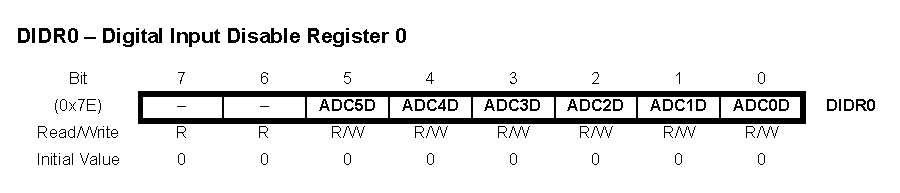
\includegraphics[width = \textwidth]{Graphics/MICROS/Practice 3/DATASHEET/DIDR0.pdf}
    \caption{Digital Input Disable Register 0~\autocite{ATMEGA328P}}
    \label{fig:DIDR0}
\end{figure}

\begin{itemize}
    \item \textbf{Bit [5:0] – [ADC5D:ADC0D]: ADC5..0 Digital Input Disable} $\bm{\rightarrow}$ When this bit is written logic one, the digital input buffer on the corresponding ADC pin is disabled. The corresponding PIN register bit will always read as zero when this bit is set. When an analog signal is applied to the ADC5..0 pin and the digital input from this pin is not needed, this bit should be written logic one to reduce power consumption in the digital input buffer. Note that ADC pins ADC7 and ADC6 do not have digital input buffers, and therefore do not require digital input disable bits.
\end{itemize}

\clearpage

\subsection{Exercise 1: Temperature measurement using LM35 sensor}

Now that we have established the basics of registers and peripherals, we can move on to solving the proposed exercise. To do so, we will use the ADC to read the output voltage of an LM35, a well-known temperature sensor. This voltage will be proportional to the ambient temperature. By perfoming some basic calculations with the read voltage, we will display it in an array of 7-segment displays. For more information on 7-segment displays, see \textbf{Section \ref{sec:7_SEG_DISP}}. \medskip

To control the 4 7-segment displays we will use a driver similar to the 4511, the one that we used in \textbf{Section \ref{sec:KEYPAD_CONTROL_VHDL}}. In this case, the driver is the 74HC595, an 8-bit serial-in parallel out shift register (See \textbf{Section \ref{sec:SHIFT_REGISTERS}} for more on this topic).\medskip

A library, the \textit{7SEG\_HC595.h}, will be used to simplify the coding. This library will take care of the communication between the ATMega328P and the 4 7-segment displays.\medskip

A basic explanation of this library can be found below:

\inputCcode{CODES/MICROS/Practice_3/EXPLANATION/74HC595.c}

The proposed code can be found below:

\inputCcode{CODES/MICROS/Practice_3/PRACTICE/LM35.c}

\clearpage

As we can see, we firstly write the necessary bits to the corresponding registers in order to enable the ADC on pin ADC4, in this case with a prescaler of 128. After that we enable the interrupts, the ADC conversion and we initialize the 4 7-segment displays.\medskip

Every time that an interrupt occurs, the ADC reading is translated into a voltage using a simple equation and it is separated into ones, tenths and hundreds using the modulus operator and some basic algebra. After separating the digits, they are individually written to the displays, with the first of them turned OFF due to the limitiation of 5 V on the input terminal of the ADC. \medskip

To simulate the circuit, we have, once again used ISIS Proteus. A small animation can be seen below:


\begin{figure}[H]
    \centering
 
    \ifnum\value{ANIMATION}=1 {
        \animategraphics[controls,loop, width = \textwidth]{1}{Graphics/MICROS/Practice 3/ANIMATION/F}{0}{3}
    } 
    \else {
        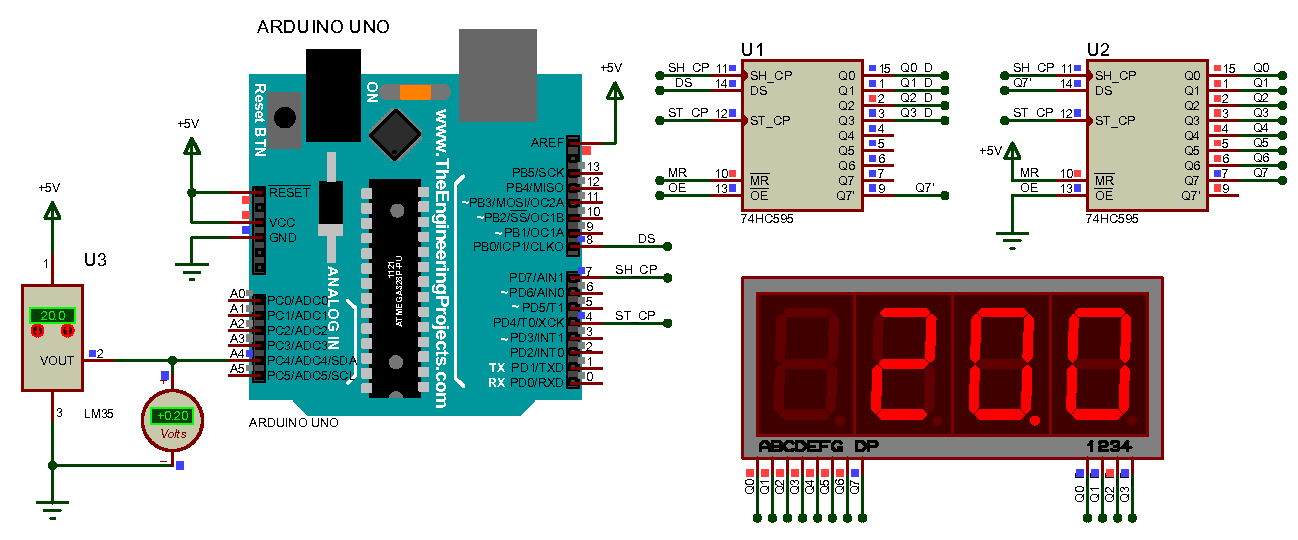
\includegraphics[width = \textwidth]{Graphics/MICROS/Practice 3/ANIMATION/F2.PDF}
    }\fi
    
    \caption{Proteus Simulation}
    \label{fig:LM35_PROTEUS_MICROS}
\end{figure}


\clearpage

